\section{Análise descritiva dos lobistas}
\label{sec:resultados_descritica_lobistas}
A Tabela \ref{tab:dist_orgs_reunioes} apresenta a distribuição de lobistas e sua atividade (mensurada pelo número de reuniões) por categoria organizacional. Os dados revelam uma predominância de interesses empresariais, que constituem o maior grupo tanto em número de organizações (2.409) quanto em volume de reuniões (22.427). Em média, cada organização empresarial realizou 9,31 reuniões, a maior taxa entre as categorias. As ONGs figuram como o segundo grupo mais ativo, seguidas pela categoria "Outros".

\begin{table}[!htbp]
\centering
\caption{Distribuição de organizações, reuniões e reuniões por lobista, por categoria de organização}
\label{tab:dist_orgs_reunioes}
\begin{tabular}{lccc}
\hline
Categoria & Organizações & Reuniões & Reuniões por Organização \\
\hline
Empresarial & 2.409 & 22.427 & 9,31 \\
ONGs & 1.271 & 10.966 & 8,63 \\
Outros & 1.042 & 6.950 & 6,67 \\
\hline
Total & 4.722 & 40.343 & 8,54 \\
\hline  
\end{tabular}
\end{table}

Esses resultados corroboram uma vasta literatura que aponta para a assimetria de recursos e representação no universo do lobby. Interesses empresariais, que dispõem de maiores recursos financeiros, tendem a predominar na atividade de lobby \cite{de_figueiredo_advancing_2014}. No contexto específico da União Europeia, estudos demonstram que grupos empresariais e associações nacionais são os mais presentes \cite{dur20212wholobbies, eising2007institutional}, o que levou alguns autores a caracterizarem o sistema como um "pluralismo de elite" \cite{coen1997evolution, schmidt2006procedural}.

A intensidade da atividade, refletida no elevado número total de reuniões (40.343), sinaliza uma forte competição pelo acesso aos tomadores de decisão, um recurso considerado escasso pela literatura \cite{hall1990buying}. Embora os atores empresariais detenham a dianteira, a presença expressiva de ONGs indica um ambiente competitivo, e não monolítico. Essa coexistência sugere que diferentes tipos de organizações mobilizam recursos distintos para influenciar o processo político. Enquanto interesses empresariais podem alavancar recursos financeiros e expertise técnica, ONGs e outros grupos da sociedade civil podem recorrer a recursos como legitimidade, representatividade e apoio público para defender suas causas \cite{Coen2019, dur_measuring_2008}.

Portanto, a análise descritiva inicial já delineia uma das tensões centrais investigadas neste trabalho: o desequilíbrio de poder e recursos entre interesses empresariais e outros setores da sociedade, e como essa assimetria se manifesta na competição por influência política no Parlamento Europeu.


% Análise do orçamento máximo declarado
A análise do orçamento máximo declarado por categoria (Figura \ref{fig:budget_ln_boxplot}), em escala logarítmica, revela padrões distributivos distintos. O grupo empresarial, embora mais numeroso em quantidade de organizações, exibe a menor mediana de orçamento e uma distribuição notavelmente mais concentrada, o que sugere uma maior homogeneidade nos gastos com lobby declarados por essas entidades.

Em contrapartida, as ONGs e a categoria "Outros" apresentam medianas mais elevadas e uma variância substancialmente maior. Essa dispersão indica uma forte heterogeneidade interna, sugerindo a coexistência de organizações com recursos modestos e outras com orçamentos muito elevados, que influenciam a distribuição.

\begin{figure}[!htbp]
\centering
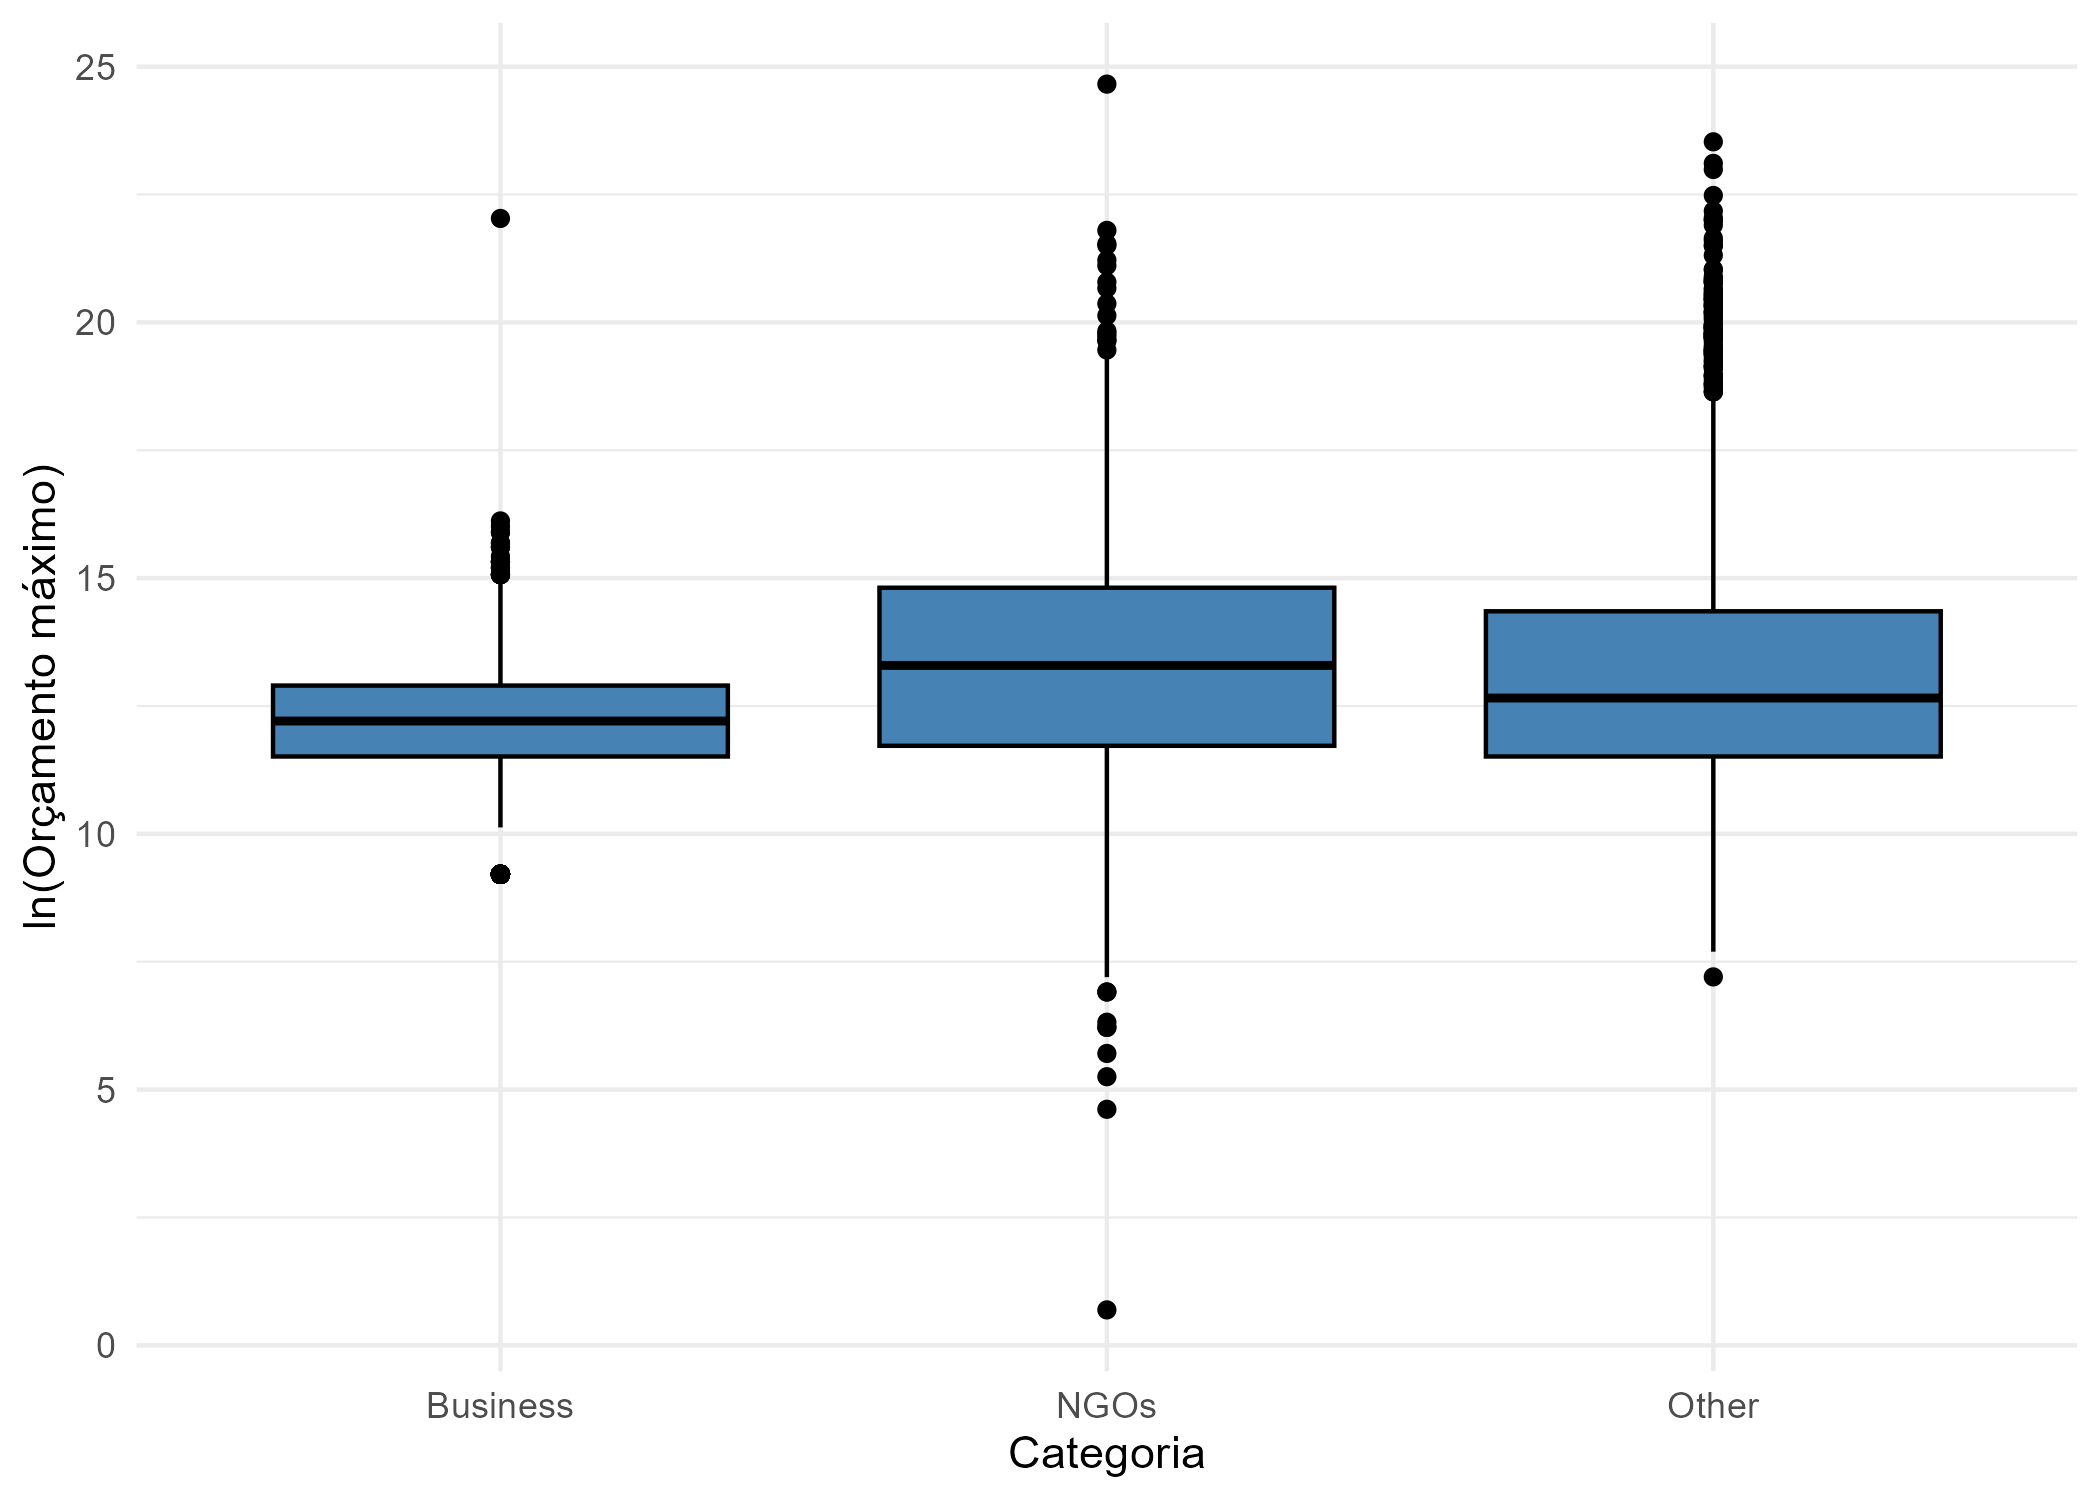
\includegraphics[width=0.75\textwidth]{figures/descriptives_lobbyists/boxplot_max_budget_by_category.png}
\caption{Distribuição de orçamento máximo declarado (\textit{ln(Orçamento Máximo Declarado)}) por categoria}
\label{fig:budget_ln_boxplot}
\end{figure}

Este achado é particularmente interessante, pois parece tensionar a premissa da literatura de que interesses empresariais dominam em termos de recursos financeiros \cite{de_figueiredo_advancing_2014, dur20212wholobbies}. Uma interpretação possível é que a categoria empresarial seja composta por um grande número de atores com gastos mais padronizados, enquanto as categorias de ONGs e "Outros" contêm algumas organizações "gigantes", cujos orçamentos massivos podem refletir campanhas de alto custo ou estruturas de financiamento distintas. A alta variância pode, ainda, ser um reflexo de diferentes estratégias: enquanto empresas podem ter um dispêndio mais constante, ONGs podem mobilizar grandes somas para temas de alta saliência, onde a opinião pública é um fator crucial \cite{mahoney_lobbying_2007}.

Adicionalmente, a concentração no grupo empresarial pode estar relacionada ao problema da ação coletiva \cite{olson1971logic}, onde muitas empresas optam por atuar por meio de associações — que podem estar classificadas na categoria "Outros". De todo modo, os dados reforçam que a relação entre recursos financeiros e influência não é direta \cite{simon_notes_1953}, e que a capacidade de mobilizar diferentes tipos de recursos — não apenas financeiros, mas também de legitimidade e informação \cite{Coen2019} — é central para a dinâmica do lobby na UE.


% Distribuição geográfica
A análise da distribuição geográfica dos lobistas (Figura \ref{fig:country_distribution}) revela uma acentuada concentração em polos institucionais da União Europeia, com Bélgica (24,2\%), Alemanha (15,3\%) e França (10,1\%) abrigando a maioria das organizações. Este padrão corrobora a tese da vantagem da proximidade institucional: a presença massiva na Bélgica, sede da Comissão Europeia e de grande parte das atividades do Parlamento, e na França, que sedia as sessões plenárias do Parlamento em Estrasburgo, é uma resposta estratégica à complexa governança multinível da UE \cite{richardson2000government}.

\begin{figure}[!htbp]
\centering
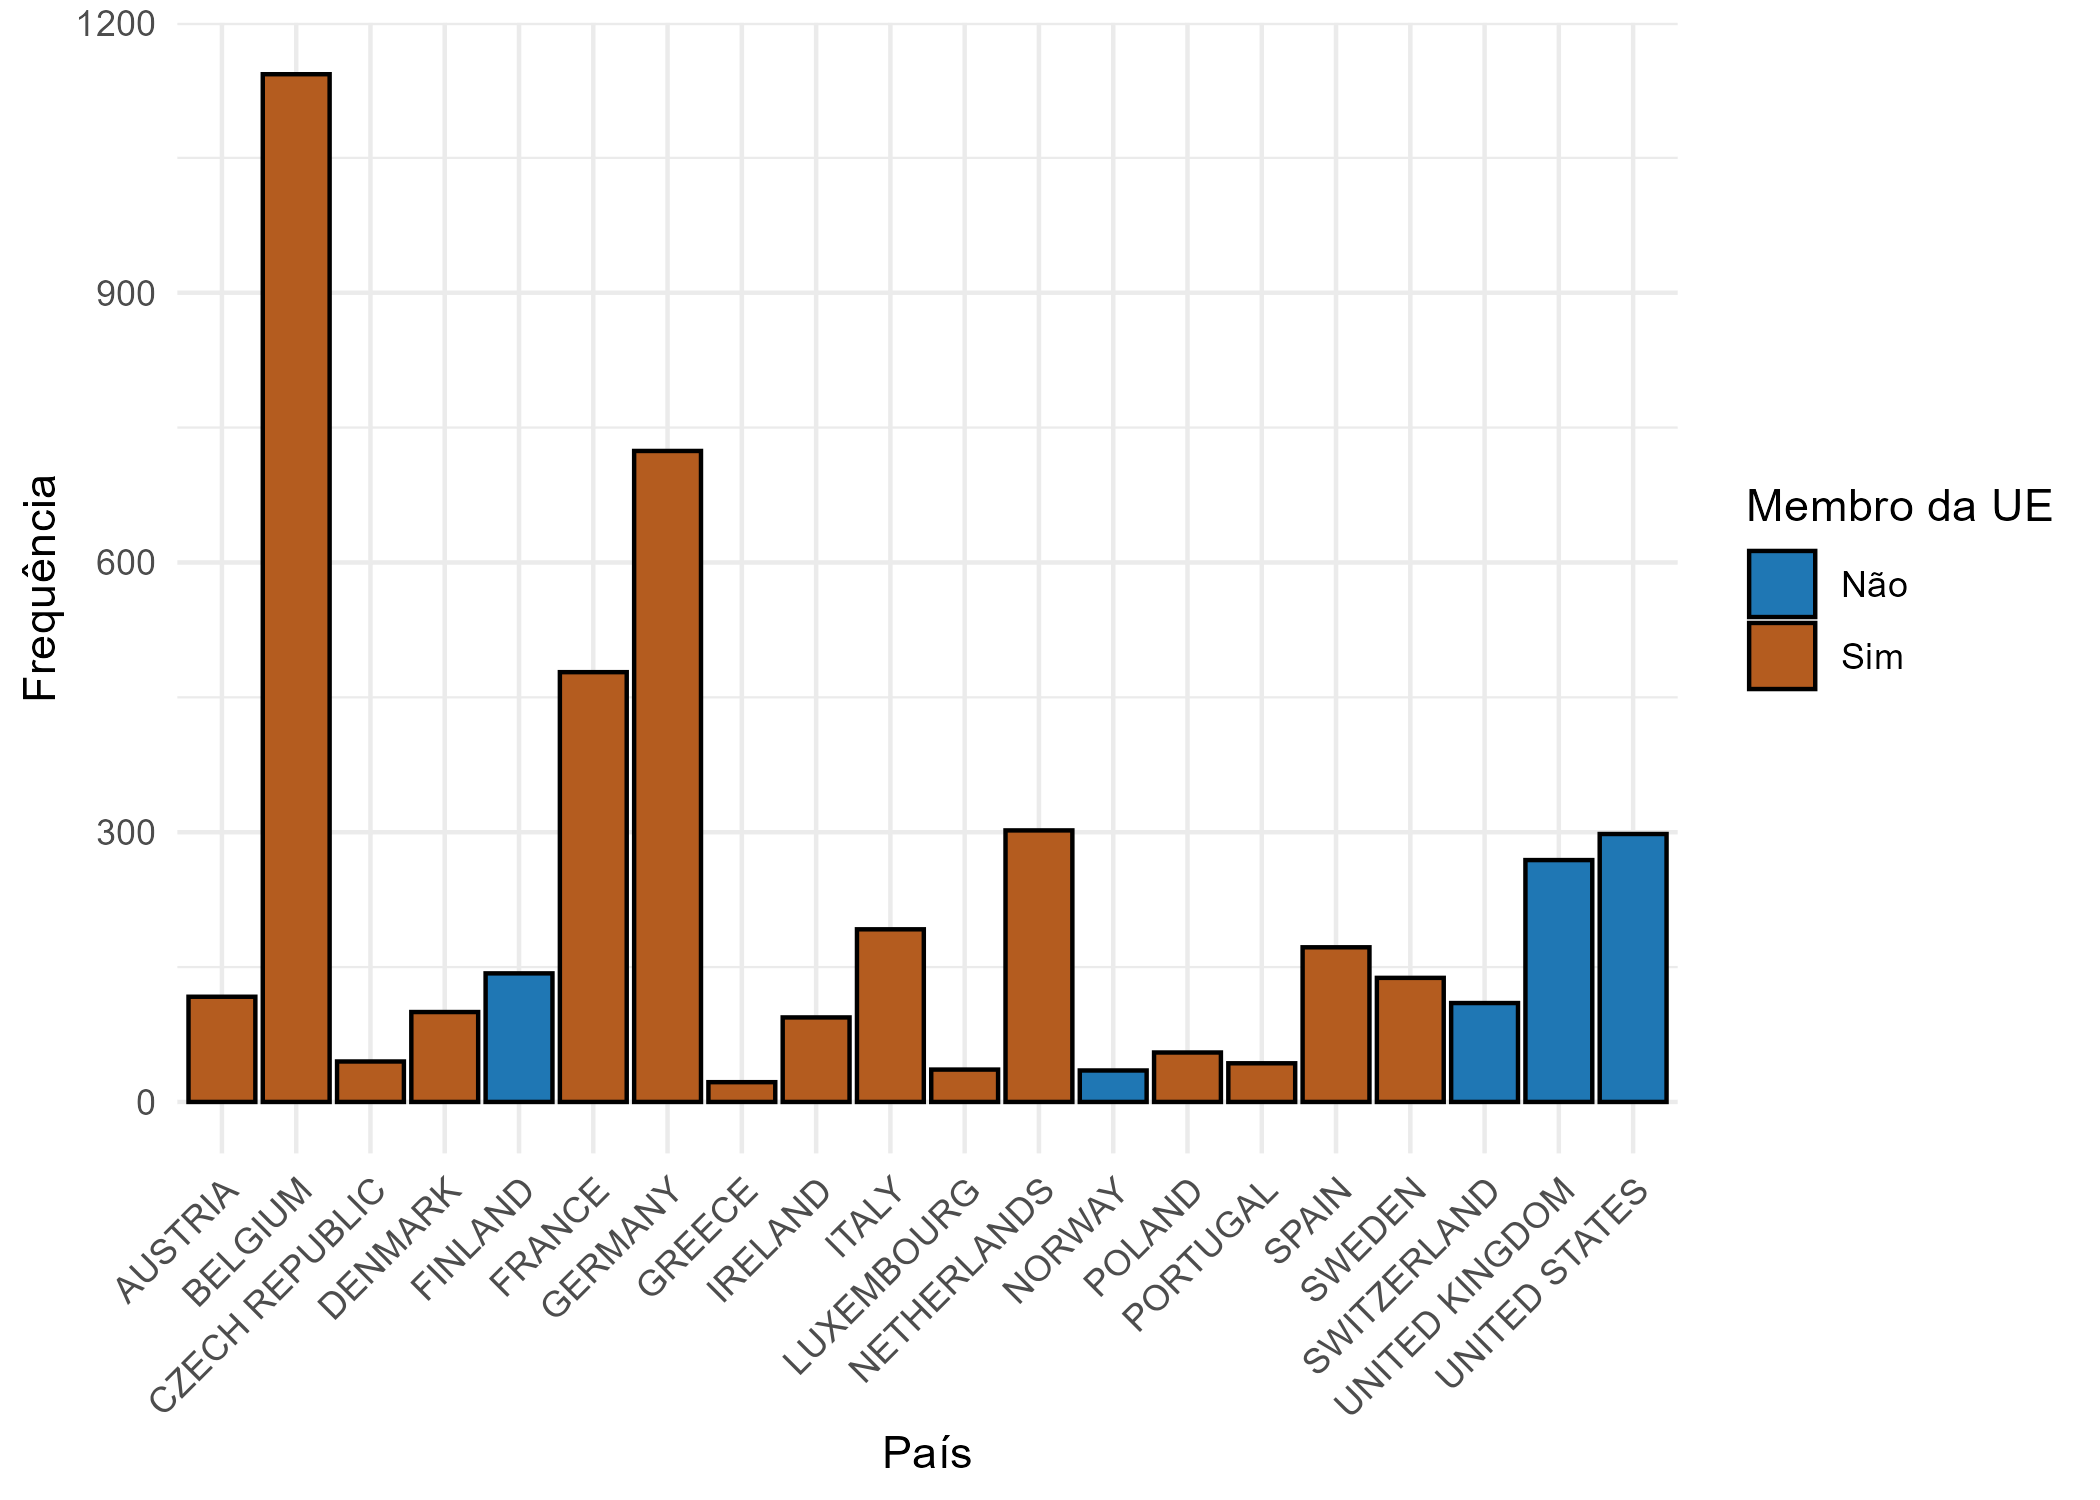
\includegraphics[width=0.9\textwidth]{figures/descriptives_lobbyists/barplot_country_distribution.png}
\caption{Top 20 países-sede (n = 4.516 organizações, totalizando 95,6\% do total de organizações)}
\label{fig:country_distribution}
\end{figure}

O fenômeno do \textit{venue-shopping} — a escolha estratégica do fórum mais favorável para exercer pressão — é central para entender essa distribuição \cite{kluver2015legislative}. A estrutura institucional da UE, com poder decisório partilhado entre a Comissão, o Conselho e o Parlamento, incentiva os grupos de interesse a se estabelecerem nos locais onde podem monitorar e intervir mais eficazmente no ciclo político. A proeminência de países como Alemanha e França reflete não apenas a proximidade, mas também o peso político e econômico que exercem dentro da União.

Adicionalmente, a presença significativa de atores extracomunitários, que representam cerca de 20\% do total de organizações com sedes em 70 países (com destaque para os Estados Unidos, com 6,3\%), evidencia a importância da UE como arena regulatória global. A atratividade do mercado europeu e o impacto de suas decisões incentivam atores internacionais a investir em uma presença local para influenciar a formulação de políticas que afetarão seus interesses. 

O recorte do top 20, que mostra uma cauda longa com muitos países de baixa frequência, reforça a ideia de que, embora o sistema seja permeável, os altos custos de manter uma operação de lobby eficaz na Europa centralizam a influência em atores com maiores recursos e localização estratégica.

% Distribuição temporal dos registros
Temporalmente, observa-se aceleração do registro de entidades após meados da década de 2010, com 2023 concentrando 17,9\% do total. Picos intermediários (2015--2016; 2020--2022) são compatíveis com ciclos legislativos, janelas regulatórias e alterações incrementais nos mecanismos de transparência.

\begin{figure}[!htbp]
\centering
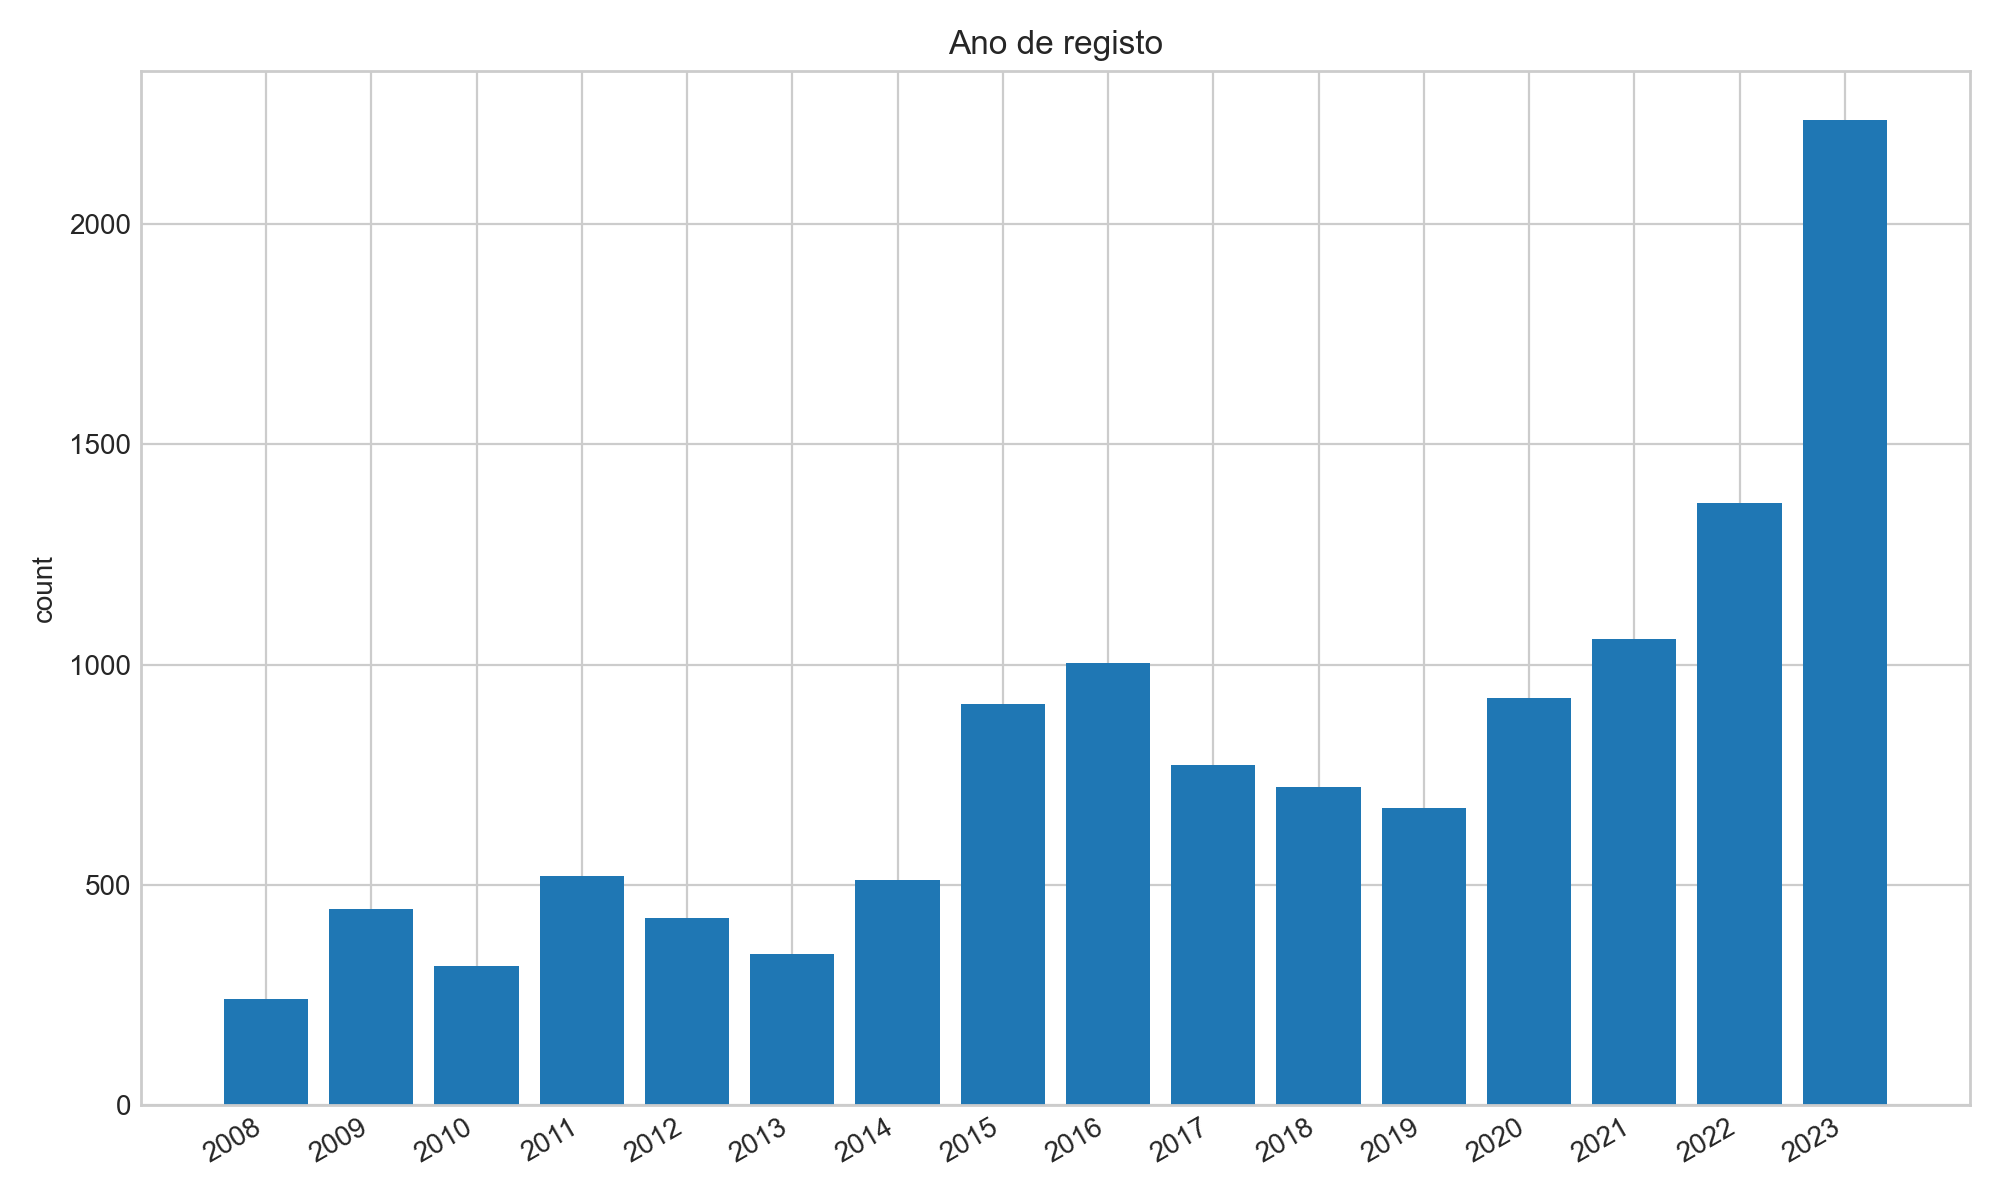
\includegraphics[width=0.75\textwidth]{figures/year_distribution.png}
\caption{Ano de registo}
\end{figure}

O padrão visual sugere crescimento estrutural recente do ecossistema de representação de interesses, possivelmente associado às agendas de transição digital e verde e à recomposição pós-pandemia.

% Distribuição temática
As incidências por domínio (Figura \ref{fig:theme_coverage}) destacam \textit{Economia e Comércio} (15\%), \textit{Tecnologia} (14,9\%) e \textit{Infraestrutura e Indústria} (14,4\%), seguidas por \textit{Tecnologia} (14,2\%) e \textit{Meio Ambiente e Clima} (13,8\%). Temas como \textit{Saúde} (9,8\%) e \textit{Educação} (8,1\%) são intermediários; \textit{Agricultura} (7,2\%) e \textit{Direitos Humanos} (6,2\%) têm menor incidência relativa.

\begin{figure}[!htbp]
\centering
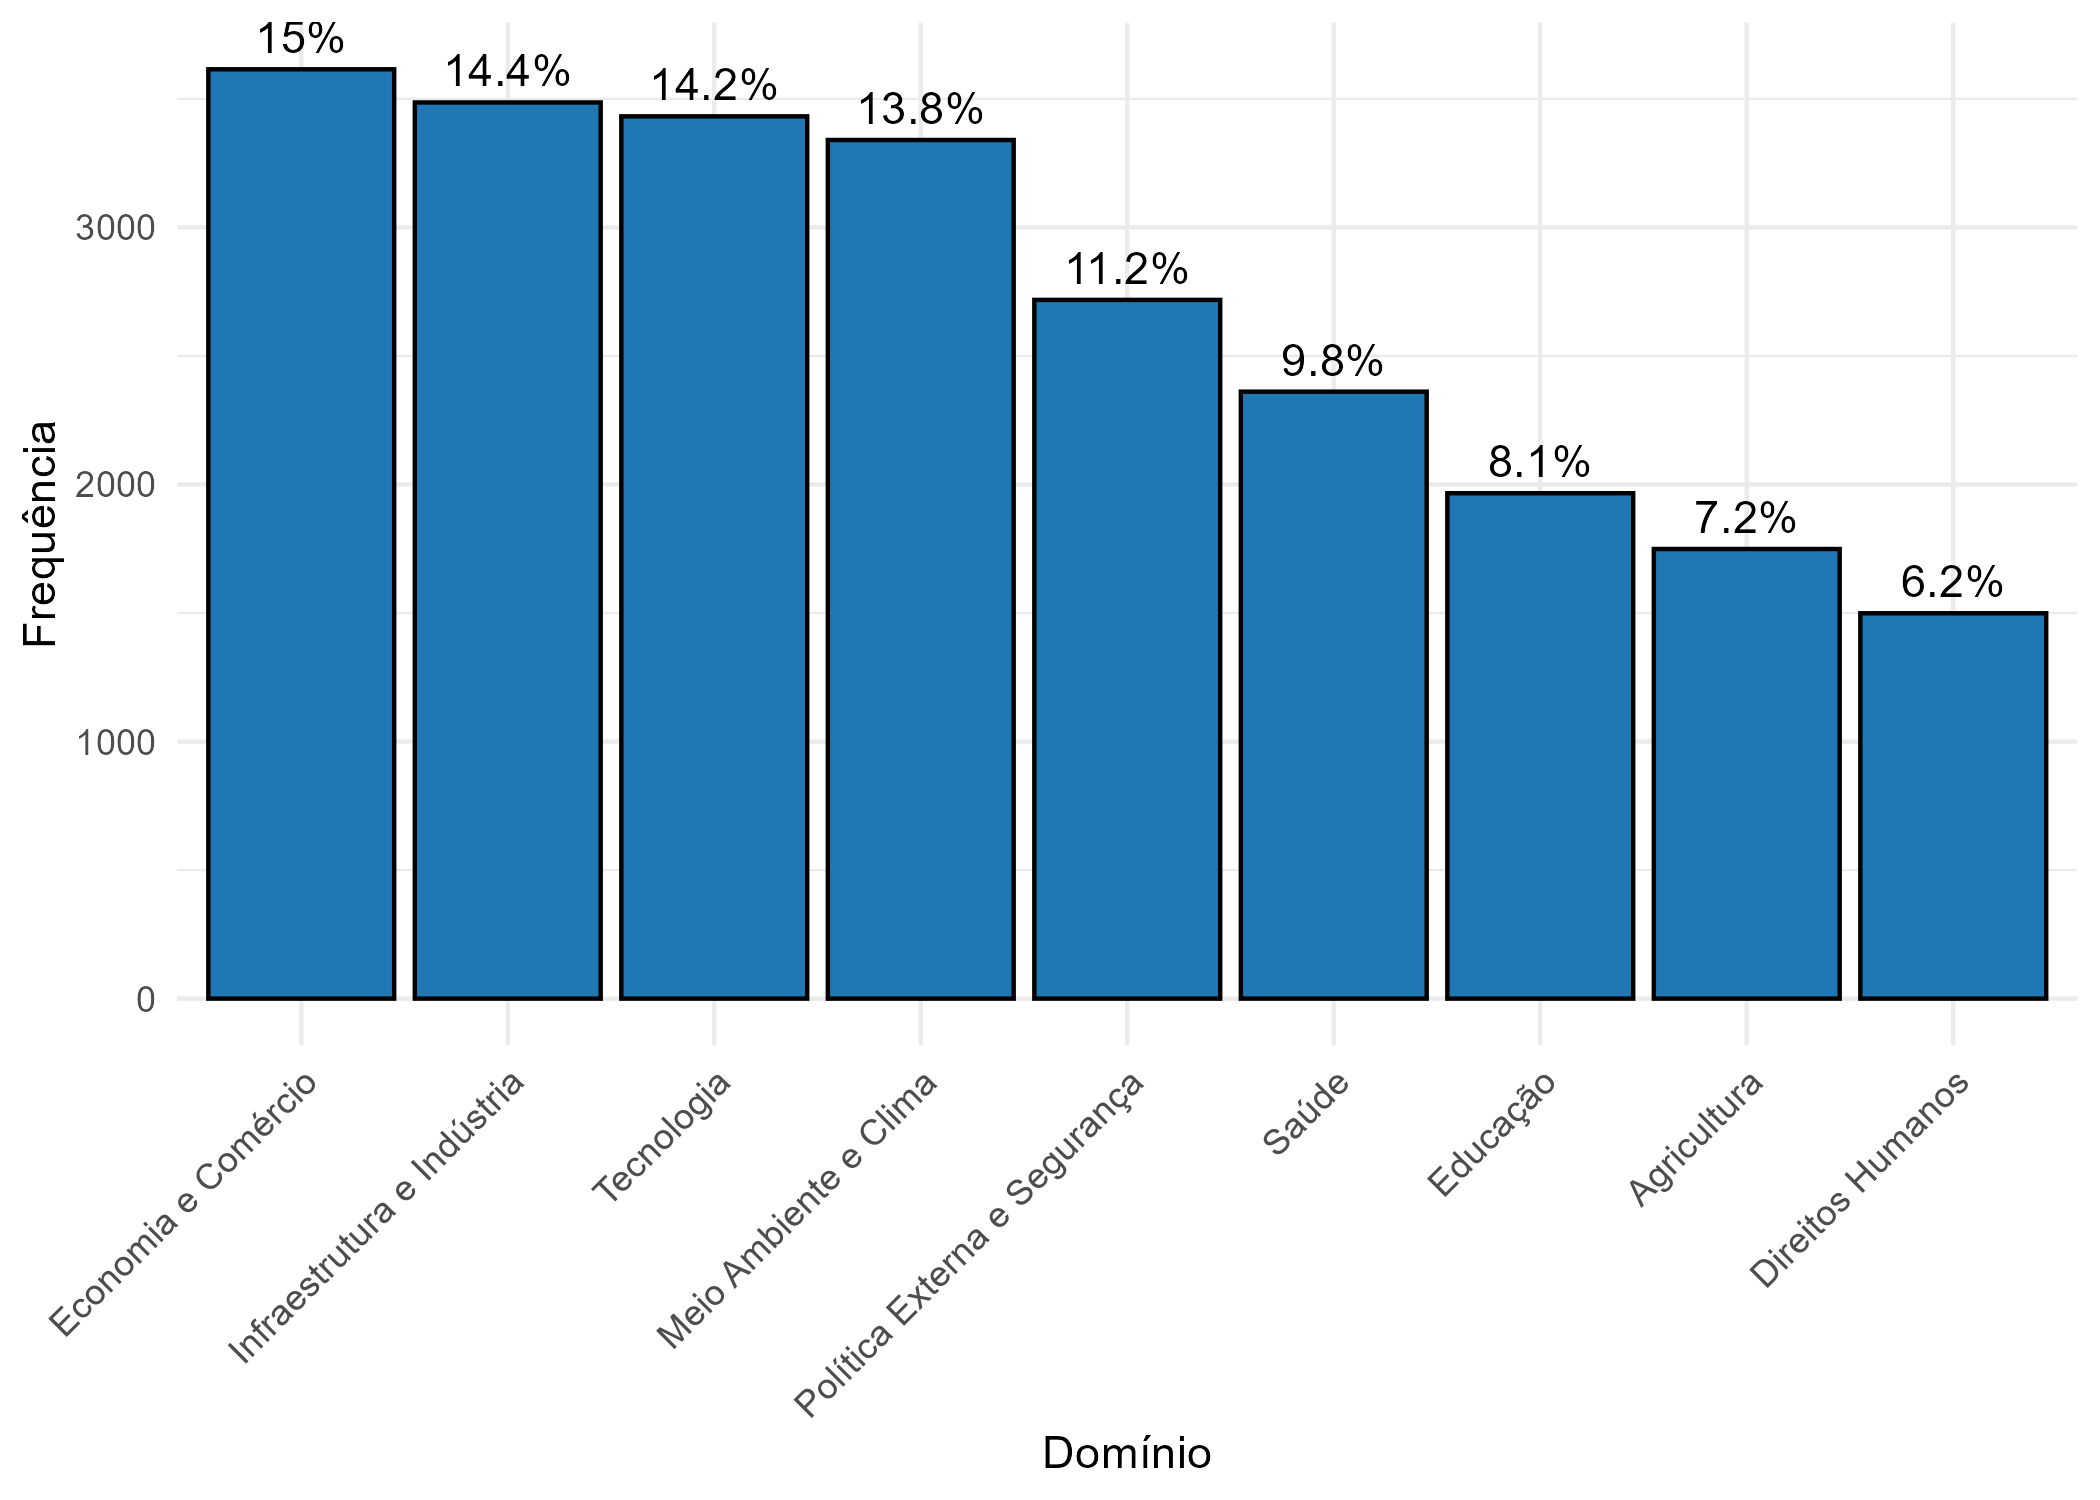
\includegraphics[width=0.9\textwidth]{figures/descriptives_lobbyists/barplot_domain_distribution.png}
\caption{Cobertura temática (proporção de entidades)}
\label{fig:theme_coverage}
\end{figure}

A distribuição temática (Figura \ref{fig:theme_coverage}) reflete uma concentração estratégica de esforços de lobby nas arenas de maior peso econômico e regulatório da União Europeia. A proeminência de domínios como "Economia e Comércio", "Infraestrutura e Indústria" e "Tecnologia" está alinhada com a literatura que demonstra uma correlação positiva entre a atividade de lobby e a saliência de um tema \cite{caldeira2000lobbying, baumgartner2010agendas}. São áreas onde as decisões políticas implicam altas consequências financeiras, mobilizando um volume expressivo de atores.

Adicionalmente, esses temas são caracterizados por uma elevada complexidade técnica. Este fator aumenta a demanda por informação especializada por parte dos decisores políticos, criando um vácuo que os lobistas buscam preencher para ganhar acesso e exercer influência, conforme sugere a literatura sobre o papel informacional do lobby \cite{kluver_informational_2012}. A própria agenda política da UE, com iniciativas centrais como o Mercado Único Digital e o Pacto Ecológico Europeu, transforma esses domínios em focos de intensa atividade, corroborando a ideia de que os grupos de interesse são mais ativos nos temas em que o Estado também é mais atuante \cite{mahoney2008brussels}.

Em contraste, temas como "Direitos Humanos" e "Agricultura", embora relevantes, apresentam menor incidência relativa. Isso pode indicar que os interesses difusos ou setoriais dessas áreas enfrentam maiores desafios de ação coletiva ou utilizam estratégias de influência distintas, que não se refletem com a mesma intensidade no lobby direto. O padrão observado, portanto, sugere um ecossistema de lobby que responde de forma racional tanto aos incentivos econômicos quanto às necessidades informacionais geradas pela agenda regulatória da UE.

\begin{figure}[!htbp]
\centering
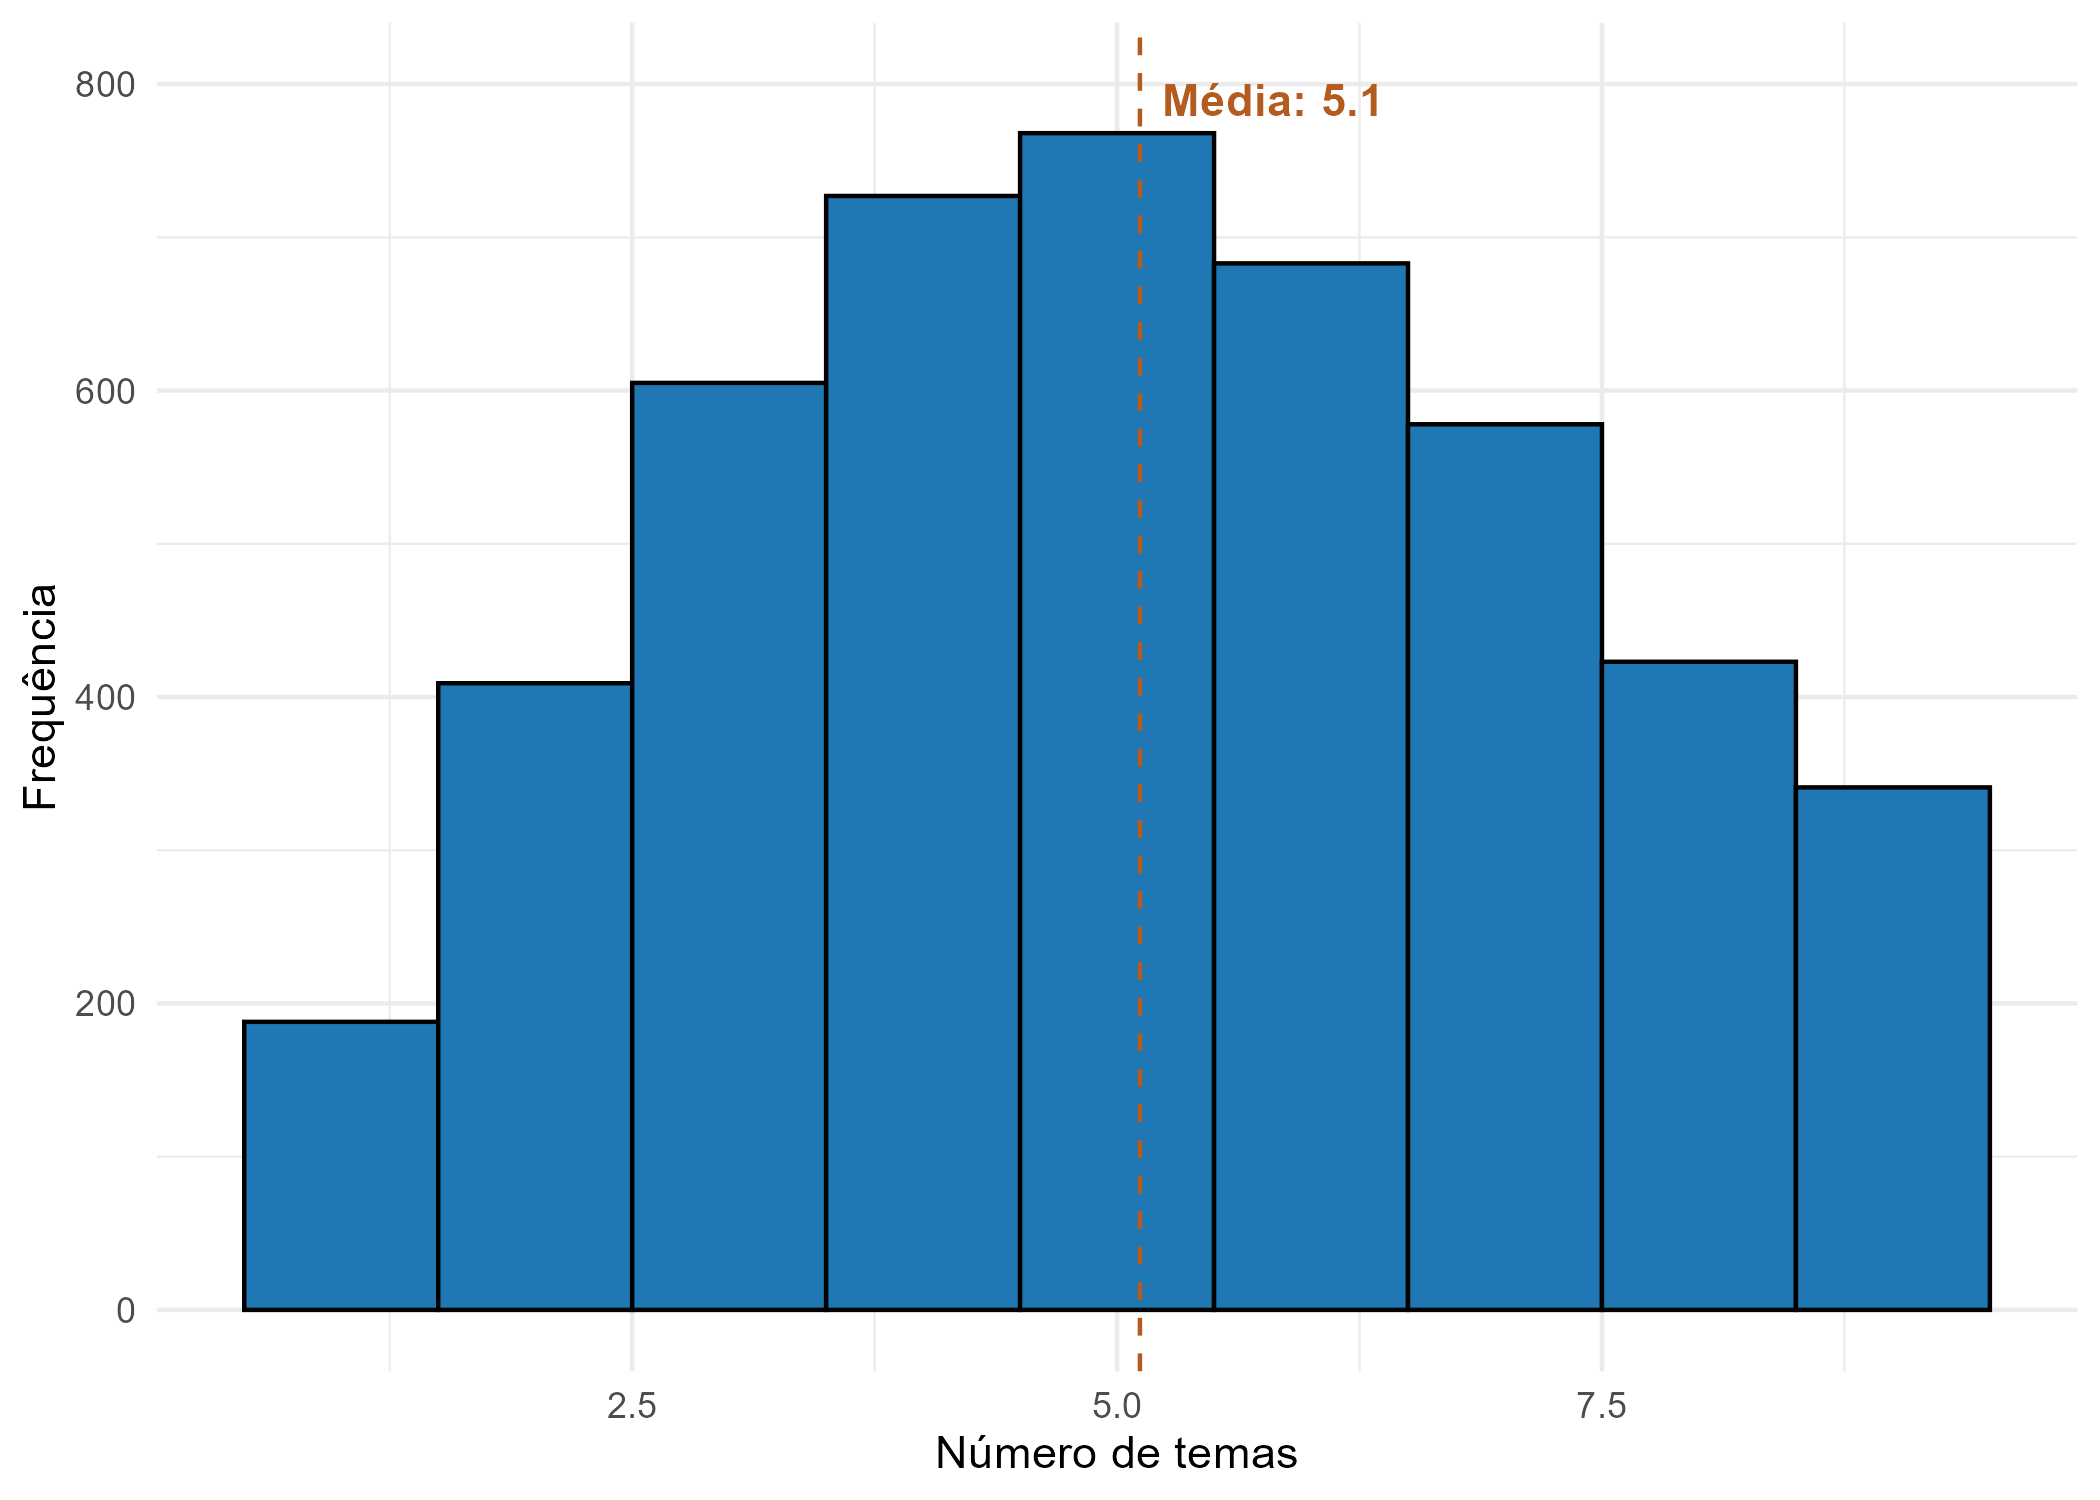
\includegraphics[width=0.75\textwidth]{figures/descriptives_lobbyists/histogram_themes_per_lobbyist.png}
\caption{Número de temas por lobista}
\label{fig:themes_per_lobbyist_hist}
\end{figure}

A análise da diversidade temática das organizações (Figura \ref{fig:themes_per_lobbyist_hist}) revela que a maioria dos lobistas atua em múltiplas frentes. A distribuição, que se assemelha a uma curva normal com média de 5,1 temas por organização, demonstra a coexistência de estratégias especializadas (focadas em poucos temas) e generalistas. Contudo, o padrão dominante é o de uma abordagem multi-temática, onde as organizações cobrem um portfólio de 3 a 7 áreas de interesse.

Este achado dialoga diretamente com o debate na literatura sobre os recursos mais valiosos para o lobby: expertise ("o que você sabe") versus conexões ("quem você conhece") \cite{bertrand2014whom}. A presença de atores especializados sugere uma aposta na expertise técnica como via de influência, especialmente em domínios de alta complexidade \cite{kluver_informational_2012}. Por outro lado, a predominância de atores multi-temáticos indica que uma estratégia mais ampla, possivelmente baseada em redes de contatos e na capacidade de adaptação a diferentes arenas políticas, é a norma no complexo ambiente institucional da UE. A governança multinível e a interconexão de políticas na Europa podem incentivar as organizações a não se limitarem a um único nicho, buscando pontos de acesso em diferentes comissões e agências \cite{coen2019legislative}.

Em conjunto, os resultados descritivos apontam para um ecossistema plural, geograficamente ancorado em polos institucionais centrais, com dinamismo temporal recente e agendas orientadas por digitalização, competitividade industrial e sustentabilidade. Esses padrões informam as escolhas de especificação nos capítulos seguintes, notadamente a estratificação por perfis organizacionais, a construção de domínios temáticos e o controle para tendências temporais.


Os resultados descritivos delineiam um panorama abrangente do universo de lobistas registados junto às instituições europeias. Em primeiro lugar, a distribuição por categoria revela a coexistência de diferentes perfis organizacionais (\textit{Empresas}, \textit{\acrshort{ong}s} e \textit{Outros}), com magnitudes comparáveis entre atores empresariais e organizações da sociedade civil. Essa composição é compatível com a literatura sobre pluralismo organizacional e competição por acesso institucional no contexto da União Europeia, sugerindo um campo de ação onde interesses difusos e concentrados buscam simultaneamente agenda e influência.

Em síntese, as evidências descritivas apontam para um ecossistema plural, geograficamente ancorado em polos institucionais centrais, com dinamismo temporal recente e agendas orientadas por digitalização, competitividade industrial e sustentabilidade. Esses padrões informam as escolhas de especificação nos capítulos seguintes, notadamente a estratificação por perfis organizacionais, a construção de domínios temáticos e o controle para tendências temporais.

